\documentclass[a4paper,14pt]{article}

\usepackage{comment} % Para comentar várias linhas ao mesmo tempo

%matemática
\usepackage{amsmath}
\usepackage{amssymb}

%diagramação
\usepackage{extsizes}
\everymath{\displaystyle}
\usepackage{geometry}
\usepackage{fancyhdr}
\usepackage{multicol}
\usepackage{graphicx}
\usepackage[brazil]{babel}
\usepackage[shortlabels]{enumitem}
\usepackage{cancel}
\usepackage{textcomp}
\usepackage{tcolorbox}

%tabelas
\usepackage{array} % Para melhor formatação de tabelas
\usepackage{longtable}
\usepackage{booktabs}  % Para linhas horizontais mais bonitas
\usepackage{float}   % Para usar o modificador [H]
\usepackage{caption} % Para usar legendas em tabelas
\usepackage{wrapfig} % Para usar tabelas e figuras flutuantes
\usepackage{xcolor} % Para cores do fundo de tabelas
\usepackage{colortbl} % Para cores do fundo de tabelas

%tikzpicture
\begin{comment}
	\usepackage{tikz}
	\usepackage{scalerel}
	\usepackage{pict2e}
	\usepackage{tkz-euclide}
	\usetikzlibrary{calc}
	\usetikzlibrary{patterns,arrows.meta}
	\usetikzlibrary{shadows}
	\usetikzlibrary{external}
\end{comment}


%pgfplots
\usepackage{pgfplots}
\pgfplotsset{compat=newest}
\usepgfplotslibrary{statistics}
\usepgfplotslibrary{fillbetween}

%colours
\usepackage{xcolor}



\columnsep=2cm
\hoffset=0cm
\textwidth=8cm
\setlength{\columnseprule}{.1pt}
\setlength{\columnsep}{2cm}
\renewcommand{\headrulewidth}{0pt}
\geometry{top=1in, bottom=1in, left=0.7in, right=0.5in}

\pagestyle{fancy}
\fancyhf{}
\fancyfoot[C]{\thepage}

\begin{document}
	
	\noindent\textbf{6FMA87 - Matemática} 
	
	\begin{center}Construção de ângulos (Versão estudante)
	\end{center}
	
	\noindent\textbf{Nome:} \underline{\hspace{10cm}}
	\noindent\textbf{Data:} \underline{\hspace{4cm}}
	
	%\section*{Questões de Matemática}
	
	\begin{multicols}{2}
		\noindent Algumas definições: \\
		\begin{table}[H]
			\begin{tabular}{|p{37mm}|p{37mm}|}
				\hline
				\textbf{Conceito} & \textbf{Condição} \\ \hline
				Ângulos complementares & Se, e somente se, a soma de suas medidas é 90°. \\ \hline
				Ângulos suplementares & Se, e somente se, a soma de suas medidas é 180° \\ \hline
			\end{tabular}
		\end{table}
		\begin{itemize}
			\item Bissetriz: \\
			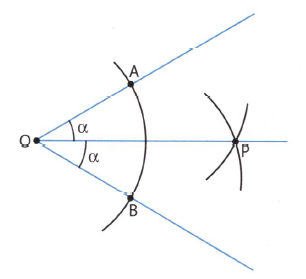
\includegraphics[width=1\linewidth]{6FMA87_imagens/imagem1}
			\item Ângulo de 30°: \\
			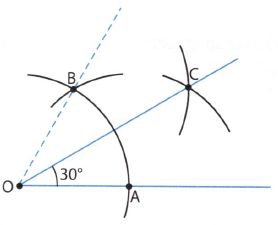
\includegraphics[width=1\linewidth]{6FMA87_imagens/imagem2}
			\item Ângulo de 60°: \\
			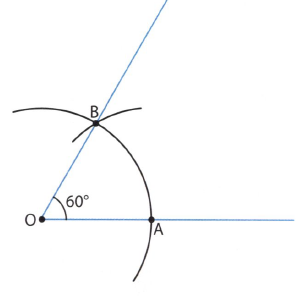
\includegraphics[width=1\linewidth]{6FMA87_imagens/imagem3}
			\item Ângulo de 45°: \\
			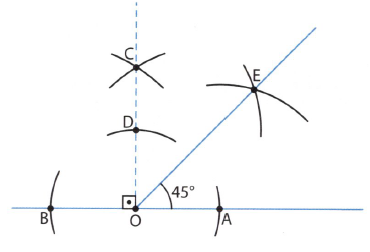
\includegraphics[width=1\linewidth]{6FMA87_imagens/imagem4}
		\end{itemize}
		\noindent\textsubscript{-----------------------------------------------------------------------}
		\begin{enumerate} 
			\item Trace as bissetrizes dos seguintes ângulos e meça com o transferidor os ângulos obtidos. \\
			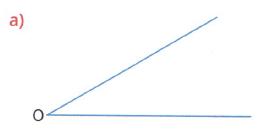
\includegraphics[width=1\linewidth]{6FMA87_imagens/imagem5}
			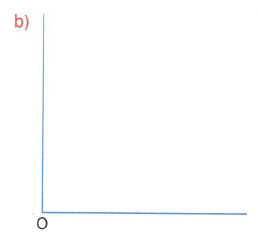
\includegraphics[width=1\linewidth]{6FMA87_imagens/imagem6}
			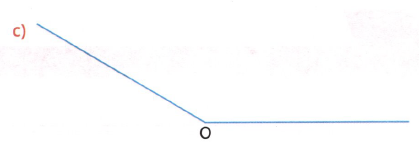
\includegraphics[width=1.1\linewidth]{6FMA87_imagens/imagem7}
			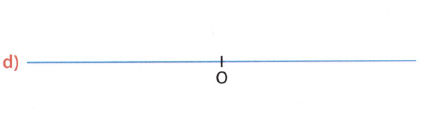
\includegraphics[width=1.1\linewidth]{6FMA87_imagens/imagem8} \\
			\item Construa com régua e compasso os ângulos e indique seu ângulo complementar ou suplementar, conforme pedido. \\
				\begin{enumerate}[a)]
					\item 60°; complementar. \\\\\\\\\\\\\\\\\\\\\\\\
					\item 90°; suplementar. \\\\\\\\\\\\\\\\\\\\\\\\\\\\
					\item 45°; complementar. \\\\\\\\\\\\\\\\\\\\\\\\\\\\
					\item 120°; suplementar. \newpage
				\end{enumerate}
			%51 a 56
			\item Construa com régua e compasso as bissetrizes dos seguintes ângulos e meça em graus, com um transferidor, os ângulos obtidos. \\
			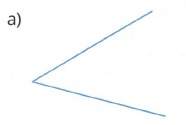
\includegraphics[width=1\linewidth]{6FMA87_imagens/imagem9}
			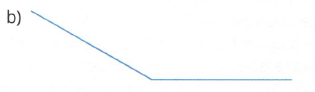
\includegraphics[width=1\linewidth]{6FMA87_imagens/imagem10}
			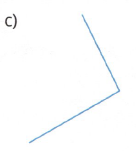
\includegraphics[width=1\linewidth]{6FMA87_imagens/imagem11}
			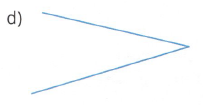
\includegraphics[width=1\linewidth]{6FMA87_imagens/imagem12} \\\\\\\\
			\item Desenhe, usando régua e compasso, um triângulo $ABC$ onde $AB$ = 6 cm, $BC$ = 9 cm e $m(\hat{B}) = 45$°. Qual a medida do terceiro lado? \\\\\\\\\\\\\\\\\\\\\\\\\\\\\\\\\\
			\item Construa, com régua e compasso, o triângulo $ABC$, sabendo que $AB$ = 6 cm, $m(\hat{A})$ = 60° e $m(\hat{B}) = 45$°. \\\\\\\\\\\\\\\\\\\\\\\\\\\\
			\item Usando a régua e o compasso, construa um triângulo que tem um lado de 7 cm e ângulos adjacentes a esse lado de medidas 30° e 60°. Qual é a medida do lado oposto ao ângulo de 30°? \\\\\\\\\\\\\\\\\\\\\\\\\\\\
			\item Usando régua e compasso, no seu caderno, desenhe um triângulo que tem um lado de 8 cm, outro lado de 9 cm e o ângulo entre eles é o complementar de 60°. Qual é a medida do terceiro lado? \\\\\\\\\\\\\\\\\\\\\\\\\\\\
			\item Desenhe, com régua e compasso, um triângulo cuja base mede 10 cm, os ângulos adjacentes a esse lado medem 15° e o ângulo oposto a esse lado é o suplementar de 30°. \\\\\\\\\\\\\\\\\\\\\\\\\\\\
			
		\end{enumerate}
		$~$ \\ $~$ \\ $~$ \\ $~$ \\ $~$ \\ $~$ \\ $~$ \\ $~$ \\ $~$ \\ $~$ \\ $~$ \\ $~$ \\ $~$ \\ $~$ \\ $~$ \\ $~$ \\ $~$ \\ $~$ \\ $~$ \\ $~$ \\ $~$
	\end{multicols}
\end{document}